%%
%% Beginning of file 'sample.tex'
%%
%% Modified 2015 December
%%
%% This is a sample manuscript marked up using the
%% AASTeX v6.x LaTeX 2e macros.

%% AASTeX is now based on Alexey Vikhlinin's emulateapj.cls 
%% (Copyright 2000-2015).  See the classfile for details.
%%
%% AASTeX requires revtex4-1.cls (http://publish.aps.org/revtex4/) and
%% other external packages (latexsym, graphicx, amssymb, longtable, and epsf).
%% All of these external packages should already be present in the modern TeX 
%% distributions.  If not they can also be obtained at www.ctan.org.

%% The first piece of markup in an AASTeX v6.x document is the \documentclass
%% command. LaTeX will ignore any data that comes before this command. The 
%% documentclass can take an optional argument to modify the output style.
%% The command below calls the preprint style  which will produce a tightly 
%% typeset, one-column, single-spaced document.  It is the default and thus
%% does not need to be explicitly stated.
%%

%% using aastex version 6
\documentclass[onecolumn]{aastex6}
\usepackage{subfigure}
\usepackage{amsmath}

%% The other main article choice is a tightly typeset, two-column article
%% that more closely resembles the final typeset pdf article.
%%
%% \documentclass[twocolumn]{aastex6}
%% 
%% There are other optional arguments one can envoke to allow other 
%% actions. 
%%
% These are the available options:
%   manuscript	: onecolumn, doublespace, 12pt fonts
%   preprint	: onecolumn, single space, 10pt fonts
%   preprint2	: twocolumn, single space, 10pt fonts
%   twocolumn	: a two column article. Probably not needed, but here just in case.
%   onecolumn	: a one column article; default option.
%   twocolappendix: make 2 column appendix
%   onecolappendix: make 1 column appendix is the default. 
%   astrosymb	: Loads Astrosymb font and define \astrocommands. 
%   tighten	: Makes baselineskip slightly smaller
%   times	: uses times font instead of the default
%   linenumbers	: turn on lineno package.
%   trackchanges : required to see the revision mark up and print output
%   numberedappendix: Labels appendix sections A, B, ... This is the default.
%   appendixfloats: Needed. Resets figure and table counters to zero

%% these can be used in any combination, e.g.
%%
%% \documentclass[twocolumn,twocolappendix,linenumbers,trackchanges]{aastex6}

%% If you want to create your own macros, you can do so
%% using \newcommand. Your macros should appear before
%% the \begin{document} command.
%%
\newcommand{\vdag}{(v)^\dagger}
\newcommand\aastex{AAS\TeX}
\newcommand\latex{La\TeX}

%% AASTeX 6.0 supports the ability to suppress the names and affiliations
%% of some authors and displaying them under a "collaboration" banner to
%% minimize the amount of author information that to be printed.  This 
%% should be reserved for articles with an extreme number of authors.
%%
%% Mark up commands to limit the number of authors on the front page.
\AuthorCallLimit=2
%% Will only show Schwarz & Muench since Schwarz and Muench
%% are in the same \author call. 
\fullcollaborationName{The Friends of AASTeX Collaboration}
%% will print the collaboration text after the shortened author list.
%% These commands have to COME BEFORE the \author calls.
%%
%% Note that all of these author will be shown in the published article.
%% This feature is meant to be used prior to acceptance to make the
%% front end of a long author article more manageable.
%% Use \allauthors at the manuscript end to show the full author list.

%% The following command can be used to set the latex table counters.  It
%% is needed in this document because it uses a mix of latex tabular and
%% AASTeX deluxetables.  In general it should not be needed.
%\setcounter{table}{1}

%%%%%%%%%%%%%%%%%%%%%%%%%%%%%%%%%%%%%%%%%%%%%%%%%%%%%%%%%%%%%%%%%%%%%%%%%%%%%%%%
%%
%% The following commented section outlines numerous optional output that
%% can be displayed in the front matter or as running meta-data.
%%
%% You can insert a short comment on the title page using the command below.
%% \slugcomment{Not to appear in Nonlearned J., 45.}
%%
%% If you wish, you may supply running head information, although
%% this information may be modified by the editorial offices.
%%\shorttitle{\aastex sample article}
%%\shortauthors{Schwarz et al.}
%%
%% You can add a light gray and diagonal water-mark to the first page 
%% with this command:
%% \watermark{text}
%% where "text", e.g. DRAFT, is the text to appear.  If the text is 
%% long you can control the water-mark size with:
%% \setwatermarkfontsize{dimension}
%% where dimension is any recognized LaTeX dimension, e.g. pt, in, etc.
%%
%%%%%%%%%%%%%%%%%%%%%%%%%%%%%%%%%%%%%%%%%%%%%%%%%%%%%%%%%%%%%%%%%%%%%%%%%%%%%%%%

%% This is the end of the preamble.  Indicate the beginning of the
%% paper itself with \begin{document}.

\begin{document}

%% LaTeX will automatically break titles if they run longer than
%% one line. However, you may use \\ to force a line break if
%% you desire.

\title{HW 05: Image Photometry}

%% Use \author, \affil, plus the \and command to format author and affiliation 
%% information.  If done correctly the peer review system will be able to
%% automatically put the author and affiliation information from the manuscript
%% and save the corresponding author the trouble of entering it by hand.
%%
%% The \affil should be used to document primary affiliations and the
%% \altaffil should be used for secondary affiliations, titles, or email.

%% Authors with the same affiliation can be grouped in a single
%% \author and \affil call.
\author{Bryan Yamashiro\altaffilmark{1}}
\author{Bryant Higa\altaffilmark{2}}
\affil{University of Hawaii at Manoa \\
2500 Campus Road \\
Honolulu, HI 96822}


%% Use the \and command so offset the last author.

%% Notice that each of these authors has alternate affiliations, which
%% are identified by the \altaffilmark after each name.  Specify alternate
%% affiliation information with \altaffiltext, with one command per each
%% affiliation.

\altaffiltext{1}{A cool dude}
\altaffiltext{2}{Another cool dude}


%% From the front matter, we move on to the body of the paper.
%% Sections are demarcated by \section and \subsection, respectively.
%% Observe the use of the LaTeX \label
%% command after the \subsection to give a symbolic KEY to the
%% subsection for cross-referencing in a \ref command.
%% You can use LaTeX's \ref and \label commands to keep track of
%% cross-references to sections, equations, tables, and figures.
%% That way, if you change the order of any elements, LaTeX will
%% automatically renumber them.

%% We recommend that authors also use the natbib \citep
%% and \citet commands to identify citations.  The citations are
%% tied to the reference list via symbolic KEYs. The KEY corresponds
%% to the KEY in the \bibitem in the reference list below. 
\section{Introduction}
The variable represent another kind of unusual star. As in the case of the peculiar stars, the variables are normal stars in special stages of their lifetimes, where particular combinations of atmospheric pressure and ionization conditions produce instabilities that cause the pulsations\,(\cite{1}).
\\
\indent Evidence of the variability of Young Stellar Object\,(YSO) J161420.3-190648\,(J-star,$\star$), a T Tau-type star, is discussed in this study. J-star is characterized as a classical T Tauri star\,(CTTS) which exhibit variability in stochastic light curves\,(\cite{2}). J-star, located at RA/Dec 16h\,14m\,20.3s -19d\,06m\,48.1s, features a literature R-magnitude of 13.2 and a K5 spectral type\,(\cite{3}). The young T Tauri stars show variations on timescales of minutes to years, but vary from object to object\,(\cite{6}). 
\\
\indent The variability of object J-star, was determined by analyzing the magnitude over time. J-star was compared to a standard star\,(J-standard,$\dagger$), 16h\,14m\,20.912s -19d\,06m\,04.70s, which has a literature apparent R-magnitude of 13.5. Measurements were carried out on a set of nine images of varying dates and times. Each image contains fully reduced observations in R from the Las Cumbres Observatory Global Telescope\,(LCOGT) 1\,m telescope network.


\section{Relevant Equations}
\indent The flux of both J-star\,(F$_{\star}$) and J-standard\,(F$_{\dagger}$), provided in equation\,\ref{flux}, were obtained with background subtraction, while also taking the gain\,($\xi$) into account. The total counts of photons\,(N$_{\star,\dagger}$) from the star apertures were subtracted with the total background photon counts\,(B).

\begin{equation}
F_{\star,\dagger} = (N_{\star,\dagger}\times \xi) - B\xi
\label{flux}
\end{equation}

The error associated with the flux required the same inputs as the flux, with a few additional parameters. The new parameters included the number of pixels within the aperture\,(N$_{px}$), read noise\,(R), and the standard deviation of the mean B$\xi$ component\,($\sigma_{\overline{B\xi}}$).

\begin{equation}
\sigma_{F_{\star,\dagger}} = \sqrt{\frac{N_{\star,\dagger}}{\xi} +  N_{px}(B\xi + R_{DN}^2) + N_{px}^2\sigma_{\overline{B\xi}}^2               }
\end{equation}


The \textit{magnitude difference}, provided in equation\,\ref{mageqn}, shows the magnitude and flux relationship between two stars. The apparent magnitude of J-star\,(m$_{\star}$) and the known magnitude of J-standard\,(m$_{\dagger}$) were both utilized. The equation also includes the flux ratio of both the photon fluxes F$_{\star}$ and F$_{\dagger}$. The error associated with the magnitude difference is provided in equation\,\ref{error}. 


\begin{equation}
m_{\star}=-2.5\log_{10}{\left( \frac{F_{\star}}{F_{\dagger}}\right)}+m_{\dagger}
\label{mageqn}
\end{equation}


\begin{equation}
\delta m_{\star} = \sqrt{\left(\frac{\partial m_{\star}}{\partial F_{\star}}\delta F_{\star}\right)^2 + \left(\frac{\partial m_{\dagger}}{\partial F_{\dagger}}\delta F_{\dagger}\right)^2}
\label{error}
\end{equation}


%\indent Find if the star is a variable. Purpose of study.
%\section{Observations}

%\section{Apparatus}
%Telescope information and methods in header. Think about removal in final.

\clearpage
\section{Procedure and Observed Quantities}
\subsection{Background Measurements}
Initially, a defined background for each image was processed. An aperture background point was set to a specific location, and a square aperture of 60x60 pixels was generated around the point. The portion of the image with low amounts of bright species was chosen through analyzing the image with contour levels, shown in figure\,\ref{background}. The background was arbitrarily defined as the 60x60 pixel aperture flux region that produced a standard deviation of less than 18. The aperture background point was set to 16h\,14m\,17.0692s -19d\,05m\,50.3571s for the first parsed image. Subsequently, the background apertures for all following images were automatically set through coordinate transforms of the initial background point.

\begin{figure*}[ht]
  \centering
  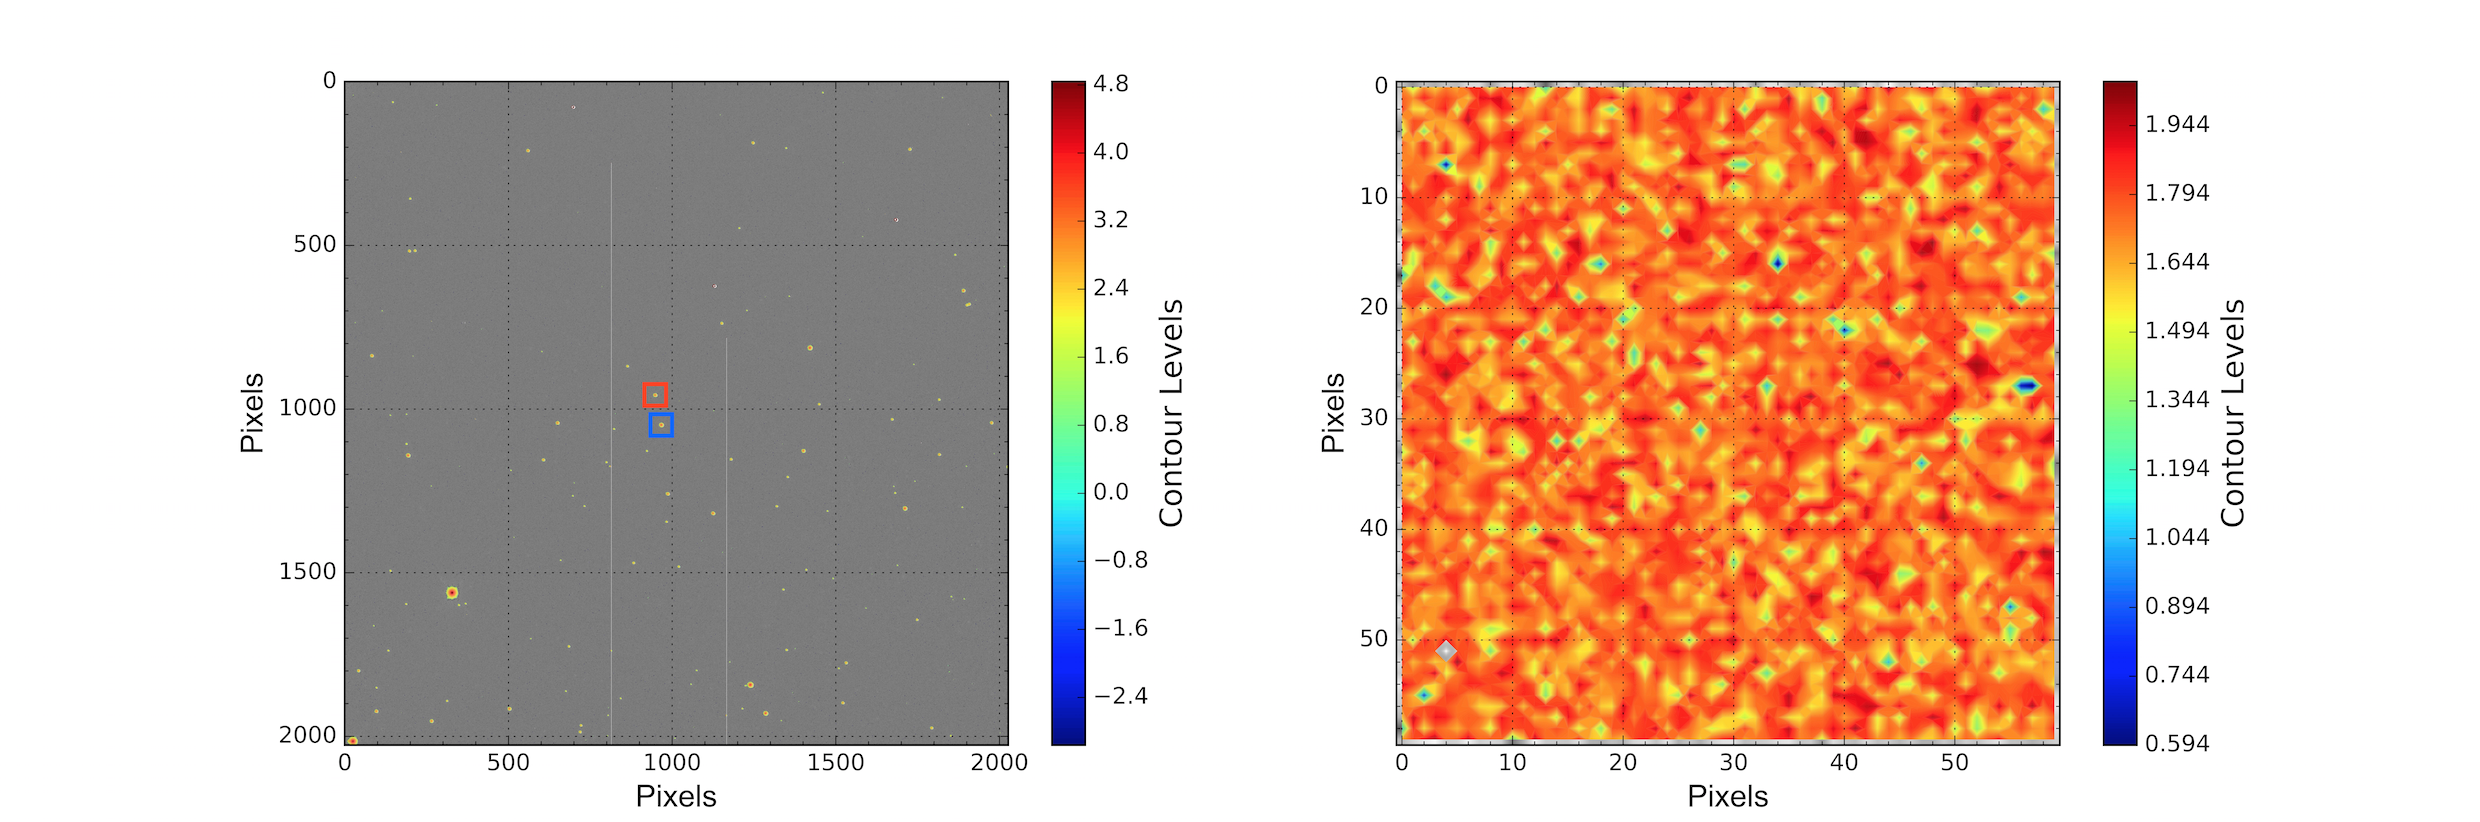
\includegraphics[scale=0.4]{background_v6.png}%\quad
  \caption{\textbf{Left:}\,The entire sky image shown with the boxed aperture regions of J-star\,(blue), J-standard\,(red), and the background\,(green). \textbf{Right:}\,The aperture region for the background image within the full-sky image. Note that the contour scales are used as a first approximation of finding a low intensity region before statistics are applied.}
  \label{background}
\end{figure*}

\subsection{J-star and J-standard Measurements}

The apertures for J-star and J-standard were generated through the same method as the background aperture. The aperture points for J-star and J-standard were 16h\,14m\,20.3s -19d\,06m\,48.1s and 16h\,14m\,20.912s -19d\,06m\,04.70s, respectively. The aperture dimensions for J-star and J-standard were set to 40x40 pixels, as this set of dimensions enclosed most of the high intensity contour levels of each star. The flux of both J-star and J-standard were measured through the dimensionally defined apertures, shown in figure\,\ref{stars}.

\begin{figure*}[ht]
  \centering
  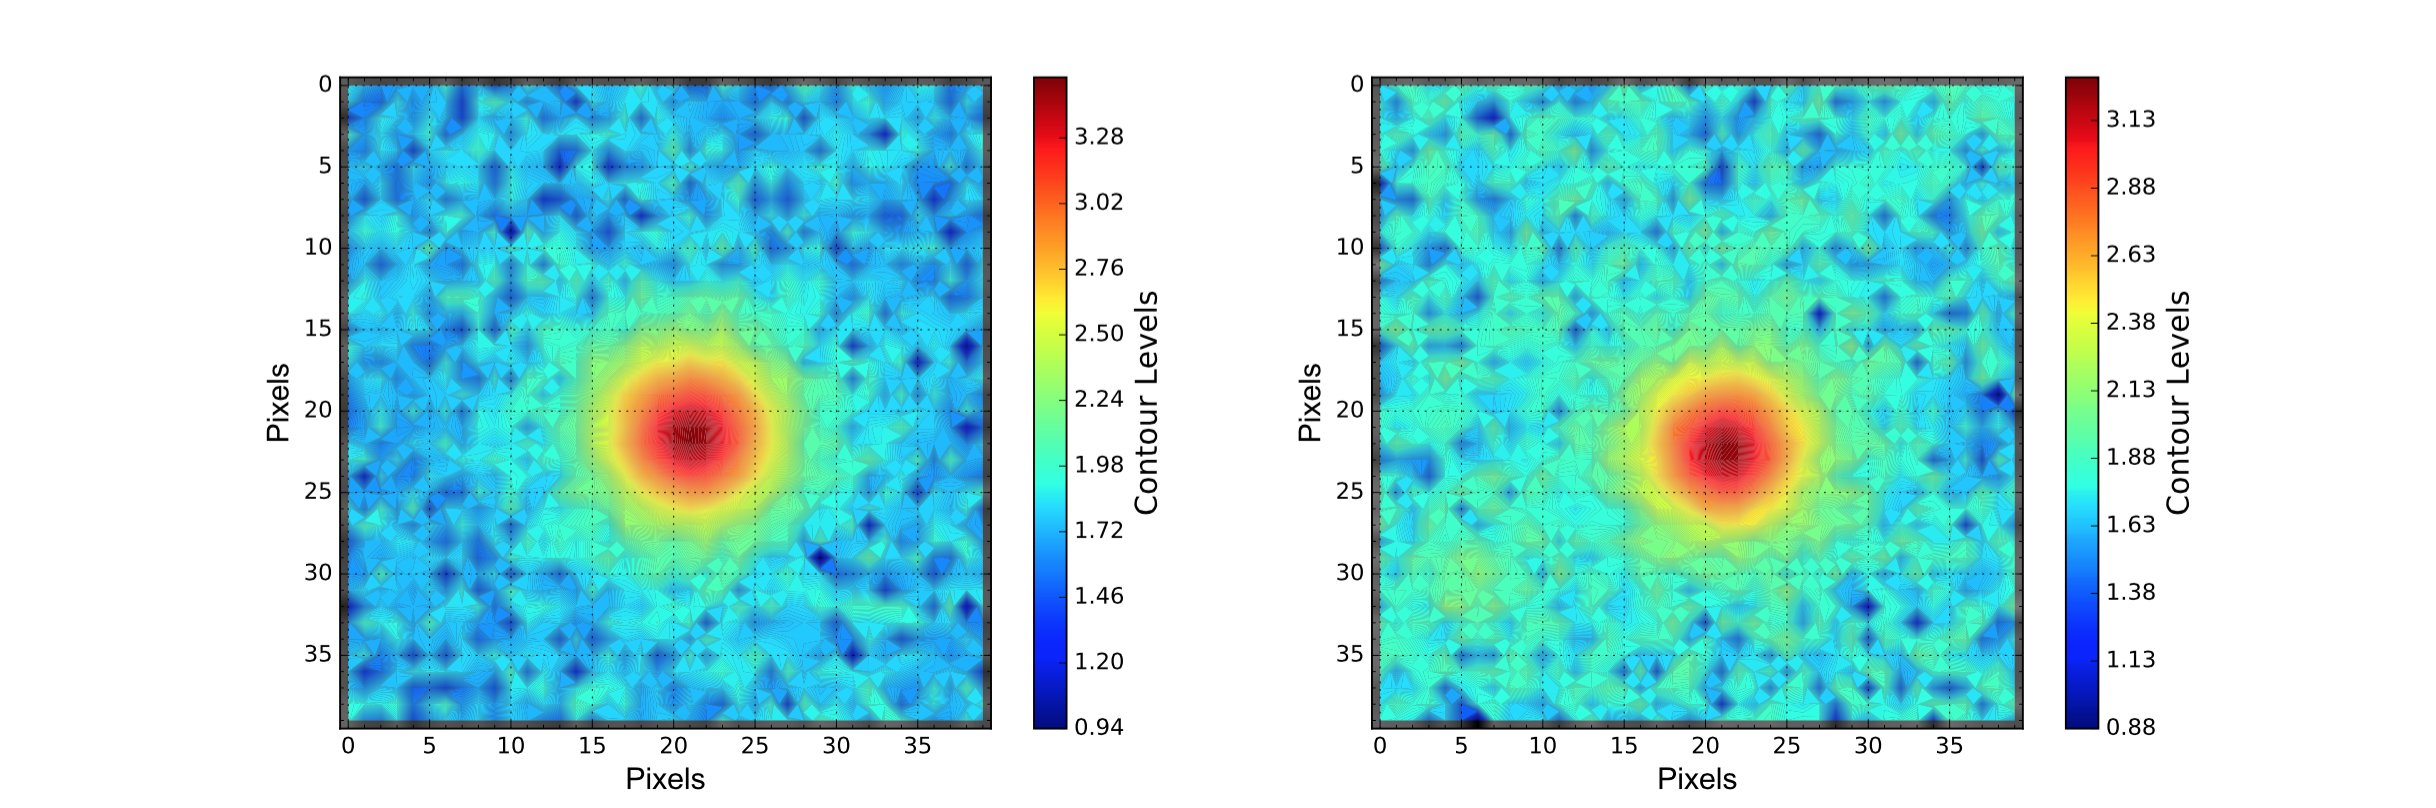
\includegraphics[scale=0.4]{star_v2.png}%\quad
  \caption{The photometric apertures containing both J-star\,(left) and J-standard\,(right). The contour levels are provided to observe the aperture localized intensities of both stars.}
  \label{stars}
\end{figure*}





%---------Procedure Notes

\clearpage
\section{Results}

\floattable
\begin{deluxetable}{cccCrlc}
\tablecaption{Apparent Magnitude Data \label{tab:mathmode}}
\tablecolumns{6}
\tablenum{2}
\tablewidth{0pt}
\tablehead{
\colhead{Observation} & \colhead{Date} & \colhead{Observation Start} & \colhead{Observation} & \colhead{F$_{\star}$} & \colhead{F$_{\dagger}$} & \colhead{m$_{\star}$} \\
\colhead{Number} & \colhead{[YYYY-mm-dd]} & \colhead{[UT]} & \colhead{Site ID} & \colhead{} & \colhead{} & \colhead{}  }
\startdata
1 & 2014-05-26  & 08:28:40  & cpt & 7940.341   $\pm$ 561.242 &  17379.420  $\pm$ 567.217 & 14.350   $\pm$ 0.085\\
2 & 2014-05-26  & 08:37:51  & cpt & 6813.614   $\pm$ 566.692 &  17511.252  $\pm$ 573.394 & 14.525   $\pm$ 0.097\\
3 & 2014-06-07  & 07:55:38  & cpt & 101939.352 $\pm$ 659.018 &  79653.540  $\pm$ 646.828 & 13.232   $\pm$ 0.011\\
4 & 2014-06-07  & 14:27:58  & elp & 80274.873  $\pm$ 711.150 &  79750.813  $\pm$ 710.887 & 13.493   $\pm$ 0.014\\
5 & 2014-06-07  & 22:19:14  & coj & 152179.862 $\pm$ 725.397 &  90519.662  $\pm$ 694.375 & 12.936   $\pm$ 0.010 \\
6 & 2014-06-07  & 22:33:39  & coj & 112276.488 $\pm$ 777.333 &  95102.906  $\pm$ 769.403 & 13.320   $\pm$ 0.012\\
7 & 2014-06-07  & 22:34:10  & coj & 116910.639 $\pm$ 770.964 &  98636.746  $\pm$ 762.452 & 13.315   $\pm$ 0.011\\
8 & 2014-06-23  & 16:14:55  & lsc & 129502.242 $\pm$ 783.233 &  201560.828 $\pm$  827.958 & 13.980  $\pm$ 0.008\\
9 & 2014-06-25  & 15:59:51  & lsc & 135379.422  $\pm$ 817.565 &  239263.188 $\pm$  878.804 &  14.118  $\pm$ 0.008\\
%2014-06-25  & 15:59:51  & lsc & 32613.693  $\pm$ 752.681 &  122060.992 $\pm$  809.923 & 14.933  $\pm$ 0.026\\
\enddata
%\tablenotetext{a}{At exposure start.}
\tablecomments{The times and dates represent the start of the observations. The flux measurements of J-star and J-standard were determined through aperture photometry. Magnitudes of J-star determined from magnitude and flux relationships are reported.}
\label{fluxtable}
\end{deluxetable}

The various flux and apparent R-magnitude aperture photometry measurements for each of the nine images are provided in table\,\ref{fluxtable} and presented in figure\,\ref{magnitudeplot}. The time varying magnitudes of J-star was found utilizing equation\,\ref{mageqn} and the appropriate values in table\,\ref{fluxtable}. 


\begin{figure}[h]
  \centering
  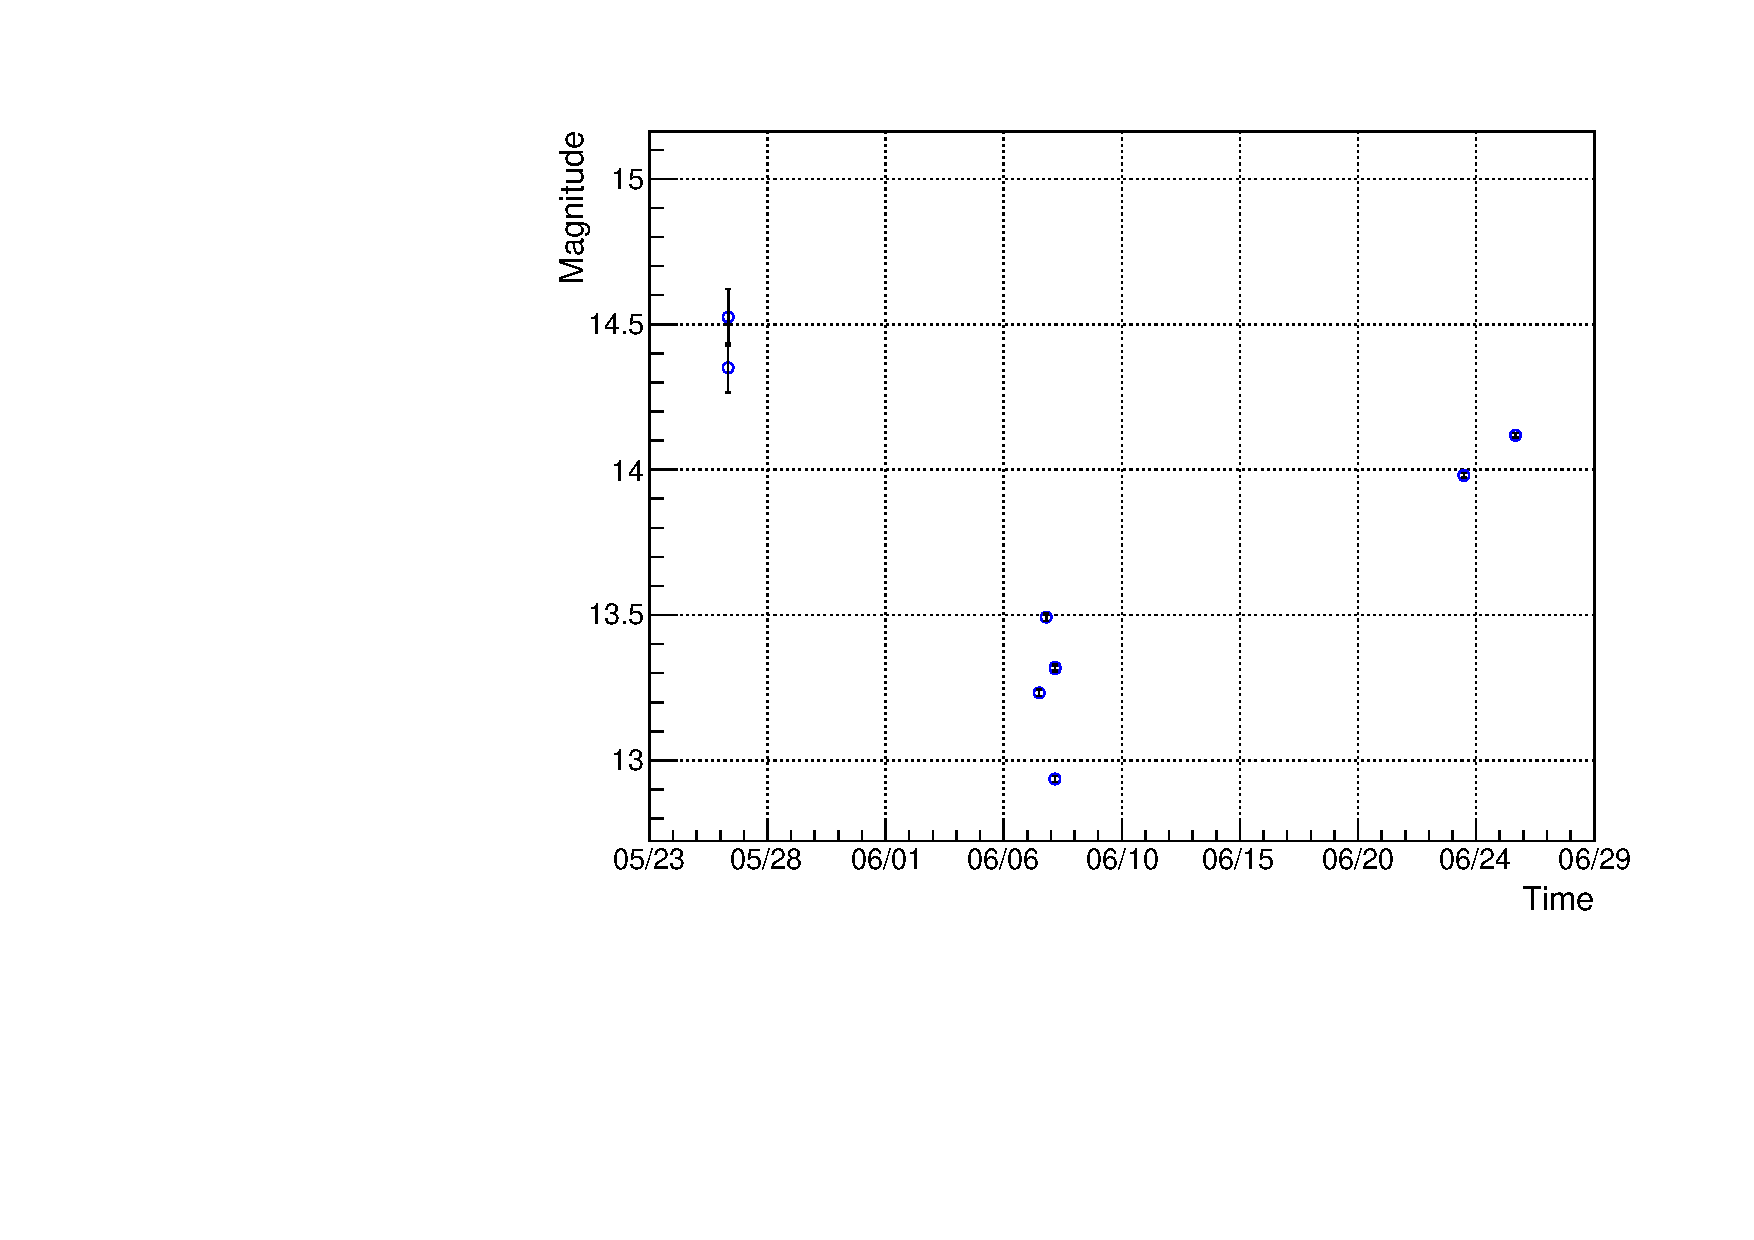
\includegraphics[scale=0.5]{magnitude.pdf}%\quad
  \caption{Magnitude diagram of J-star over approximately a month timescale. Note that observations 5 and 6 are similar in time and magnitude, therefore the points are essentially overlapping.}
  \label{magnitudeplot}
\end{figure}





\section{Discussion}
The J-star magnitude, shown in figure\,\ref{magnitudeplot}, clearly exhibits variability between approximately 13 to 14.5 magnitudes. The R-magnitude literature of 13.2 lies within this magnitude range. It is imperative to note that without additional data on a larger time range, it is impossible to definitively determine the variability of J-star. Multiple periods of the magnitude fluctuation would solidify the variability conjecture. The change in magnitude slightly followed characteristics of CTTS, as CTTS species were determined to portray rotation periods of approximately 2.8 days\,(\cite{5}).
\\
\indent J-star could more accurately be classified as an irregular variable suffering occultations\,(Type III variable) with the information provided in the study. Earlier type CTTS are thought to undergo irregular variability with brightness drops from 1 to 3 magnitudes followed by irregular recoveries.\,(\cite{5}). This characteristic is evident in figure\,\ref{magnitudeplot}, if the maximum magnitude is taken around 14.5 and the minimum magnitude is taken around 13. This assumption assumes that the period from the maximum to the minimum is approximately 14 days. Converse to the above statement, the assumption does not fully support the 2.8 day period mentioned by common CTTS objects, as the period is elongated over the span of a month. From the magnitude minimum to the last two points observations in time, the magnitudes are still low relative to the maximum magnitude with a time difference of over approximately 20 days. These traits show an antisymmetry over the total magnitude curve. A verification on the antisymmetric characteristic of a type III variable could be confirmed by magnitude measurements 14 days after the minimum, along with a longer time range. This test would confirm if there exists a magnitude maximum that is not represented by the current sample, and thus exhibiting a symmetric periodicity.

%\acknowledgments



\vspace{5mm}

\begin{thebibliography}{}


\bibitem[Cody et al.(2014)]{2}
Cody et al., 2014, Astronomical Journal, volume 147, p. 82

\bibitem[Herbst(2012)]{5}
Herbst, W. 2012, Journal of the American Association of Variable Star Observers, 40, 448

\bibitem[Gham et al.(1995)]{6}
Gahm, G. F., Loden. K. Gullbring, E., \& Hartstein, D. 1995, A\&A, 301, 89 

\bibitem[Matthews(2012)]{4}
Mathews, G. S., Williams, J. P., \& Menard, F. 2012, ´ ApJ, 753, 59

\bibitem[Preibisch(2008)]{3}
Preibisch \& Mamajek, 2008, from the book Handbook of Star Forming Regions, Volume II, ed. B. Reipurth.



\bibitem[Snow(1984)]{1}
Snow, Theodore P., and Theodore P. Snow. Essentials of the Dynamic Universe: An Introduction to Astronomy. St. Paul: West, 1984. Print.


\end{thebibliography}



%% Appendix material should be preceded with a single \appendix command.
%% There should be a \section command for each appendix. Mark appendix
%% subsections with the same markup you use in the main body of the paper.

%% Each Appendix (indicated with \section) will be lettered A, B, C, etc.
%% The equation counter will reset when it encounters the \appendix
%% command and will number appendix equations (A1), (A2), etc.


%% The reference list follows the main body and any appendices.
%% Use LaTeX's thebibliography environment to mark up your reference list.
%% Note \begin{thebibliography} is followed by an empty set of
%% curly braces.  If you forget this, LaTeX will generate the error
%% "Perhaps a missing \item?".
%%
%% thebibliography produces citations in the text using \bibitem-\cite
%% cross-referencing. Each reference is preceded by a
%% \bibitem command that defines in curly braces the KEY that corresponds
%% to the KEY in the \cite commands (see the first section above).
%% Make sure that you provide a unique KEY for every \bibitem or else the
%% paper will not LaTeX. The square brackets should contain
%% the citation text that LaTeX will insert in
%% place of the \cite commands.

%% We have used macros to produce journal name abbreviations.
%% \aastex provides a number of these for the more frequently-cited journals.
%% See the Author Guide for a list of them.

%% Note that the style of the \bibitem labels (in []) is slightly
%% different from previous examples.  The natbib system solves a host
%% of citation expression problems, but it is necessary to clearly
%% delimit the year from the author name used in the citation.
%% See the natbib documentation for more details and options.


\end{document}

%% End of file `sample.tex'.
